%!TEX root = ../main.tex


%\noindent We show how to use \cosette for debugging \jsil code annotated with 
%separation logic (SL) specifications. Tools that support SL-reasoning about
%functional correctness properties of programs often require of the user to 
%analyse long, complex proof traces whenever
%verification fails. 
%\cosette substantially simplifies this process by providing
%concrete counter-models that invalidate the input specification. 

We show how to use \cosette for debugging \jsil code annotated with separation logic (SL) specifications.
To achieve this, we extend the 
 \jsil symbolic interpreter with a mechanism for asserting
SL-assertions (\S\ref{subsec:sep:assertions}) and show how to 
implement this mechanism by giving a sound decision procedure 
for solving the frame inference problem (FIP)~\cite{berdine:aplas:2005}
in the context of symbolic execution (\S\ref{subsec:fip}).
%
%Unlike verification tools, our emphasis is in the generation of counter-models for failing cases. 
%
In \S\ref{specs:to:symbolic:tests}, we present an algorithm  
for generating symbolic tests from SL-specifications, which guarantees 
that when a symbolic test fails, \cosette produces a concrete 
counter-model that invalidates the corresponding specification. 
We conclude with a discussion on how to lift the presented results to JavaScript (\S\ref{subsec:liftmejs2}).
All definitions and proofs are given in full in the Appendix.

\vspace{-5pt}
\subsection{Symbolic Execution with SL-Assertions}\label{subsec:sep:assertions}

\jsil Logic assertions~\cite{javert} provide a way of describing \emph{partial} symbolic states.
They include boolean and comparison operations on \jsil expressions; the separating conjunction; 
and assertions for describing heaps. The $\lemp$ assertion describes 
an empty heap. The \emph{cell assertion}, $(\jsilexpr_1,\jsilexpr_2) \pointsto \jsilexpr_3$,  states that the object 
at the location denoted by $\jsilexpr_1$ has the property denoted by $\jsilexpr_2$ with value 
denoted by $\jsilexpr_3$. The \emph{object domain} assertion $\emptyfields{\jsilexpr_1}{\jsilexpr_2}$ states that the object at 
the location denoted by $\jsilexpr_1$ has \underline{at most} the properties included in the
set denoted by $\jsilexpr_2$. For instance, the assertion $\emptyfields{\sloc}{\jsilset{p_1, p_2}}$ 
states that the object at location $\sloc$ has \emph{at most} the properties $p_1$ and $p_2$; 
it might only have one of them, or none at all, but it cannot have others.
% \polish{(it may only have some of those properties but it certainly does not have any property that is not included in that set)}.  
% no properties other than possibly those included in the set denoted by $\jsilexpr_2$. 
We refer to assertions that are distinct from $\lemp$ and $- \sep -$ as \emph{simple assertions}, and use $\spass$, $\sqass$ 
to range over them.

%\pmaxinline{Mention sth about Es being the same.} %The syntax of assertions is given below. 
%We refer to assertions different from $- \sep -$ and $\lemp$ as \emph{simple assertions}
%and use $\spass$ and $\sqass$ to range over them.

\vspace{2pt}
\begin{display}{\jsil Logic Assertions}
%
{\small
\begin{tabular}{r@{\ }c@{\ }lr}
  %%%%
  %$\lexpr$ & $\triangleq$ & $\val \mid \jvar \mid \svar \mid \unoper\ \lexpr \mid \lexpr \binoper \lexpr$ & Logical Exprs. \\
  $\rass, \sass$ & $\triangleq$ & $\jtrue \mid \jfalse \mid  \neg \rass \mid \rass \land \sass \mid \rass \lor \sass \mid \jsilexpr = \jsilexpr \mid \jsilexpr \leq \jsilexpr$ & Pure Asrts. \\
  $\pass, \qass$ & $\triangleq$ & $\rass \mid \lemp \mid (\jsilexpr, \jsilexpr)\pointsto \jsilexpr \mid \pass \sep \qass \mid \emptyfields{\jsilexpr}{\jsilexpr}$ & Asrts.
\end{tabular}}
\end{display}

\noindent Without loss of generality, we implicitly assume that different symbolic locations 
denote different concrete locations. %\footnote{To express aliasing, the user has to write multiple assertions.}
 Furthermore, given a cell assertion $(\jsilexpr,-) \pointsto -$, we always assume 
 $\jsilexpr$ to be either a concrete location $\loc$ or a symbolic location $\sloc$. 
%
Note that 
a symbolic state $\sstate = (\sheap, \sdom, \sstore, \pc)$ corresponds to the assertion:
\begin{equation*}
{\small \begin{array}{l}
\big(\varoast_{(\sloc, \sexprp) \in \domain(\sheap)} (\sloc, \sexprp) \mapsto \sheap(\sloc, \sexprp)\big) 
  \sep \big(\varoast_{\sloc \in \domain(\sdom)} \, \emptyfields{\sloc}{\idom(\sloc)}\big)  \\
 %
 \qquad \sep \big(\bigwedge_{\jvar \in \domain(\sstore)} \, \jvar = \sstore(\jvar)\big) \sep \pc
\end{array}}
\end{equation*}

\noindent where $\varoast$ denotes the iterated separating conjunction~\cite{reynolds:lics:2002}. 

%\pmax{Describe this and do better on the below}

Analogously, an assertion can be normalised into a symbolic state, by:
mapping all program variables in $\pass$ to freshly generated logical variables of the appropriate type, obtaining a symbolic store~$\sstore$;
replacing all program variables in $\pass$ with their bindings given by $\sstore$, obtaining an assertion $\pass'$ with no program variables; and
 collecting all cell assertions in $\pass'$ to form the symbolic heap,
             all object domain assertions to form the domain table, and all pure assertions to form the path condition.
We refer to the normalised symbolic state corresponding to $\pass$ by $\normaliser(\pass)$. 
%
We also use $\interpret{}{}(\sstate)$ for denoting the set 
$\{ (\jstate, \heap_f) \mid \exists \senv \, . \, (\jstate, \heap_f) \in \interpret{\symbconc}{\senv}(\sstate) \}$ 
and $\interpret{}{}(\pass)$ for $\interpret{}{}(\normaliser(\pass))$. 

\myparagraph{Inductive Predicates}
\cosette does not support symbolic execution over inductive predicates, which are commonplace 
in SL-style specifications~\cite{smallf, berdine:aplas:2005}. 
As in~\cite{korat}, we deal with user-defined inductive predicates by \emph{unfolding} 
those predicates up to a fixed, user-defined bound. We omit this unfolding mechanism 
as it is routine. 

\myparagraph{Asserting SL-Assertions}
We extend \jsil commands with a special construct, $\sepassert(P)$, for stating that 
 the SL-assertion $P$ must hold whenever that command is evaluated. 
The corresponding symbolic semantics rules are given below. 

\vspace*{-0.2cm}
{\footnotesize
\begin{mathpar}
\inferrule[\textsc{SL-Assert - True}]
  { 
     \ccmd{\scs, i}  = \sepassert(\pass)  \\\\
     %
     \unificationfun(\sstate, \pass) = \success{\sstate_f}
  }{
    \abssemrule{\sstate, \scs, i}{\sstate, \scs, i{+}1}{\top}{\top}{\symbolic}
}
\qquad
\inferrule[\textsc{SL-Assert - False}]
  { 
     \ccmd{\scs, i}  = \sepassert(\pass)  \\\\
     %
    \unificationfun(\sstate, \pass) = \fail{\pc_f}  \quad
    %
     (\sstate.\pcsel \wedge \pc_f) \text{ SAT}
  }{
    \abssemrule{\sstate, \scs, i}{\sstate, \scs, i}{\top}{\bot}{\symbolic}
}
\end{mathpar}}

\vspace*{-0.2cm}
\noindent The rules use a partial decision procedure (PDP), $\unificationfun(\sstate, \pass)$, for 
determining if a given symbolic state $\sstate$ satisfies an assertion $P$. 
%which is undecidable in general \cite{citemeplease}. 
There are two important criteria that $\unificationfun(\sstate, \pass)$ must satisfy:
\begin{enumerate}[leftmargin=*]
\setlength{\itemsep}{0.1cm}
%
\item {\bfseries Soundness}: If $\unificationfun(\sstate, \pass) = \success{\sstate_f}$, then it must hold that $\interpret{}{}(\sstate) \subseteq \interpret{}{}(\sstate_f \statecompose \normaliser(\pass))$;\footnote{We use $\statecompose$ for the composition of two symbolic states, defined component-wise as disjoint union for the  heaps/domains/stores, and conjunction for the path conditions.}
%
\item {\bfseries Bug-Finding}: If $\unificationfun(\sstate, \pass) = \fail{\pc_f}$, then it must hold that $\interpret{}{}(\sstate \, \wedge \, \pc_f) \cap \interpret{}{}(\pass) = \emptyset$. Observe that every concrete state and heap frame in $\interpret{}{}(\sstate \, \wedge \, \pc_f)$ are counter-models for $P$. 
Also note that, in the \textsc{SL-Assert - False} rule, the semantics only triggers an assertion failure when it finds a concrete witness for the failure, 
as it explicitly requires that $(\sstate.\pcsel \wedge \, \pc_f)$ be satisfiable.
\end{enumerate}



\subsection{The Frame Inference Problem}\label{subsec:fip}

We describe the $\unificationfun(\sstate, \pass)$ PDP that we
use as part of the \jsil sym-bolic interpreter, for proving entailments 
between symbolic states \underline{and} finding counter 
models in case of failure.  
As is customary~\cite{javert,jacobs2011verifast,sepwithsmt}, this PDP first uses \emph{pattern-matching} 
on the spatial part of the symbolic state, and then discharges the pure part of the 
entailment to an external constraint solver (in our case, \rosette). 



When solving $\unificationfun(\sstate, \pass)$, the symbolic variables of $\pass$ that are not 
in $\sstate$ are assumed to be existentially quantified. 
As in~\cite{nguyen:vmcai:2008}, we 
topologically sort the simple assertions in $\pass$ to find the appropriate bindings 
for such variables. Here, for lack of space, we describe the frame inference 
algorithm for the setting without existentially quantified variables. 
The full version is given in the Appendix.  

Given a symbolic state $\sstate$ and an assertion $\pass$, $\unificationfun(\sstate, \pass)$ 
 replaces the program variables in $\pass$ with their bindings 
from $\sstate.\stosel$ and then calls the Frame Inference Algorithm (Algorithm~1) 
 on the list of all simple assertions in $\pass$. This algorithm uses two~functions: 

\begin{description}
\setlength{\itemsep}{0.2em}
  \item[FIP GetCell.] In case of success, $\GetCellV{\sstate, \sloc, \sexprp}$ returns 
          the symbolic expression $\sexprv$ associated with 
          $(\sloc, \sexprp)$ in the heap component of $\sstate$ \underline{and} 
          the state obtained by removing that cell from $\sstate.\hpsel$.
  
  \item[FIP GetDomain.] In case of success, $\GetDomainV{\sstate, \sloc}$ returns 
          the symbolic expression $\sexprv_d$, denoting the domain 
          of the object at location $\sloc$ in $\sstate$, \underline{and} 
          the state obtained by removing all the negative resource associated with 
          $\sloc$ from $\sstate$.  
%  
%  \item[Expression Unification.]  In case of success, $\unifylexpr(\sexprv, \sexprv', \subst, \pc)$ 
%          returns a substitution $\subst'$ that extends $\subst$ such that $\pc \vdash \sexprv = \subst'(\sexprv')$. 
\end{description}

\noindent We give selected rules for these functions, analogous to those in \S\ref{subsec:symb:semantics}, except that: \dtag{1} both functions return a new symbolic state 
from which the matched resource is removed and \dtag{2} their corresponding constraints are lifted to the premise (highlighted in blue). 
Also, in case of failure, both functions return a constraint $\pc_f$, under which the inspected resource is guaranteed not to exist (highlighted in~red). 

\smallskip
\begin{display}{Selected FIP Rules}
\text{
{\scriptsize
\begin{mathpar} 
  \inferrule[\textsc{GetDomain}]
   { 
       \sheap = \sheap' \, \uplus \, \big((\sloc, \sexprp_i) \mapsto \sexprv_i \big)\mid_{i = 0}^m  
         \quad 
          (\sloc,-) \notin \domain (\sheap')  
         \quad
        \forall_{0 \leq i \leq n} \,  \sexprv_i \neq \none 
         \quad
           \forall_{n < i \leq m} \, \sexprv_i = \none
           \\\\ 
           \sexprv =  \{ \sexprp_i \mid_{i = n{+}1}^m\}
           \and
           \sheap'' = (\sloc, \sexprp_i) \mapsto \sexprv_i  \mid_{i=0}^n
           \and
           \sdom = \sdom' \dunion (\sloc \mapsto \sexprv')
   }{  \GetDomainV{(\sheap, \sdom, \sstore, \pc), \sloc} \semeq \success{(\sexprv' \backslash \sexprv}, (\sheap' \, \uplus \,  \sheap'', \sdom', \sstore, \pc))}
  \\
      \inferrule[\textsc{GetCell - Found}]
   { 
      (\sheap, \sdom, \sstore, \pc) = \sstate    
       \quad
       \sheap = \sheap' \, \uplus \, (\sloc, \sexprp') \mapsto \sexprv 
       \\\\
       {\color{blue} \pc \vdash (\sexprp = \sexprp')}
       \quad
       \sstate' = (\sheap', \sdom, \sstore, \pc)
   }{  \GetCellV{\sstate, \sloc, \sexprp} \semeq \success{ \sexprv, \sstate'}}
\quad
     \inferrule[\textsc{GetCell - Not Found}]
   { 
     (\sheap, \sdom, \sstore, \pc) = \sstate  
     \quad 
        { \color{blue} \pc \vdash \sexprp \not\in \sdom(\sloc)}
        \\\\
        \sstate' = (\sheap, \sdom[\sloc \mapsto \sdom(\sloc) \cup \jsilset{\sexprp}], \sstore,  \pc)
   }{  \GetCellV{\sstate, \sloc, \sexprp} \semeq \success{\none, \sstate'}}
\\
     \inferrule[\textsc{GetCell - Fail with Domain Info}]
   { 
       \sheap = \sheap'' \, \uplus \, \big((\sloc, \sexprp_i) \mapsto \sexprv_i \big)\mid_{i = 0}^m
      \qquad
       (\sloc,-) \notin \domain (\sheap'')
       \qquad
        { \color{blue} \pc \not\vdash \sexprp \not\in \sdom(\sloc)}
        \qquad
          { \color{blue} \pc \not\vdash \sexprp = \sexprp_i \mid_{i=0}^m}
   }{  \GetCellV{(\sheap, \sdom, \sstore, \pc), \sloc, \sexprp} \semeq \fail{{\color{red} (\sexprp \in \sdom(\sloc)) \, \wedge \, (\wedge_{i=0}^m (\sexprp_i \neq \sexprp))}}}
 \\
     \inferrule[\textsc{GetCell - Fail without Domain Info}]
   { 
       \sheap = \sheap'' \, \uplus \, \big((\sloc, \sexprp_i) \mapsto \sexprv_i \big)\mid_{i = 0}^m
      \qquad
       (\sloc,-) \notin \domain (\sheap'')
       \qquad
       \sloc \not\in \domain(\sdom)
        \qquad
          { \color{blue} \pc \not\vdash \sexprp = \sexprp_i \mid_{i=0}^m}
   }{  \GetCellV{(\sheap, \sdom, \sstore, \pc), \sloc, \sexprp} \semeq \fail{{\color{red} \wedge_{i=0}^m (\sexprp_i \neq \sexprp)}}}
 \end{mathpar}}}
 \end{display}

\smallskip
The Frame Inference Algorithm has four possible cases: 
\begin{itemize}[leftmargin=*]
\setlength{\itemsep}{0.1cm}
\item  $\jvec{\spass}=\lstemp$~: there is nothing left to unify; we 
            return the current symbolic state, which constitutes the frame. 
   
   \item $\jvec{\spass} = (\sloc, \sexprp) \pointsto \sexprv \lstcons -$~:
            using $\GetCellVFun$, we obtain the symbolic expression~$\sexprv'$
            associated with $(\sloc, \sexprp)$ in the current symbolic state and
            check that $\sexprv' = \sexprv$ under the current path condition. 
            If the entailment holds, we proceed. Otherwise, we generate
            the \emph{failing constraint} $\sexprv' \neq \sexprv$. 
  
   \item $\jvec{\spass} = \emptyfields{\sloc}{\sexprv} \lstcons -$~:
            using $\GetDomainVFun$, we obtain the domain $\sexprv'$
            of $\sloc$ in the current symbolic state and 
            check that $\sexprv' \subseteq \sexprv$ under the current path condition. 
            %\polish{For instance, the assertion $\emptyfields{\sloc}{\jsilset{p_1, p_2}}$ states that $\sloc$ has \emph{at most} the properties $p_1$ and $p_2$. It might only have one of them, or none at all. But it cannot have more.}
            If the entailment holds, we extend the current symbolic state with the negative 
            resource associated with $\sloc$ not captured by $\emptyfields{\sloc}{\sexprv}$ and  proceed. 
            Otherwise, we generate the \emph{failing constraint} $\sexprv' \not\subseteq \sexprv$. 
            
   \item $\jvec{\spass} = \sass \lstcons -$~:  
            we check that $\sass$ is entailed by the current path condition. 
             If it is, we proceed. Otherwise, we generate
             the \emph{failing constraint} $\neg \sass$. 
\end{itemize}

%{\footnotesize \begin{algorithm}[t!]
%\algblock[Name]{match}{end}
%\caption{Frame Inference for Symbolic States}\label{fip:symb:states}
%\begin{algorithmic}[1]
%\Function{Unification}{$\sstate$, $\jvec{\spass}$}
%    \State $\textbf{match}$ $\jvec{\spass}$ $\textbf{with}$
%    \State $\mid~\lstemp:$ \Return $\success{\sstate}$
%   % Cell ASS
%    \State $\mid~(\sloc, \sexprp) \pointsto \sexprv \lstcons \jvec{\sqass} :$ 
%    \State $\qquad \textbf{match} \ \GetCellV{\sstate, \sloc, \sexprp}$ $\textbf{with}$
%    \State $\qquad \mid~\success{\sexprv', \sstate'}:$ $\textbf{if} \,(\sstate.\pcsel \vdash \sexprv = \sexprv')$
%     \State $\qquad \qquad \qquad ~  \textbf{then}$ \Return  \Call{Unification}{$\sstate'$, $\jvec{\sqass}$}
%     \State $\qquad \qquad \qquad ~  \textbf{else}$ \Return $\fail{\sexprv \neq \sexprv'}$
%      \State $\qquad \mid~\fail{\pc_f}:$ \Return $\fail{\pc_f}$
%      % EF ASS
%     \State $\mid~\emptyfields{\sloc}{\sexprv} \lstcons \jvec{\sqass} :$  
%       \State $\qquad \textbf{match} \ \GetDomainV{\sstate, \sloc}$ $\textbf{with}$
%       \State $\qquad \mid~\success{\sexprv', \sstate'}:$ $\textbf{if} \,(\sstate.\pcsel \vdash \sexprv \backslash \sexprv' = \{ \sexprp_1, ..., \sexprp_n \})$
%        \State $\qquad \qquad \qquad ~  \textbf{then}$ \Return \Call{Unification}{$\sstate' \dunion (\sloc, \sexprp_i) \pointsto \none \mid_{i = 1}^n$, $\jvec{\sqass}$}
%       \State $\qquad \qquad \qquad ~  \textbf{else}$ \Return $\fail{\sexprv' \not\subseteq \sexprv }$
%       \State $\qquad \mid~\fail{\pc_f}:$ \Return $\fail{\pc_f}$
%     % OTHER PURE ASS
%     \State $\mid~\sass \lstcons \jvec{\sqass} :$  $ \textbf{if} \,(\sstate.\pcsel \vdash \sass)$
%       \State $\qquad \qquad \textbf{then}$ \Return  \Call{Unification}{$\sstate$, $\jvec{\sqass}$}
%      \State $\qquad \qquad \textbf{else}$  \Return $\fail{\neg \sass}$
%\EndFunction
%\end{algorithmic}
%\end{algorithm}}

\begin{figure}
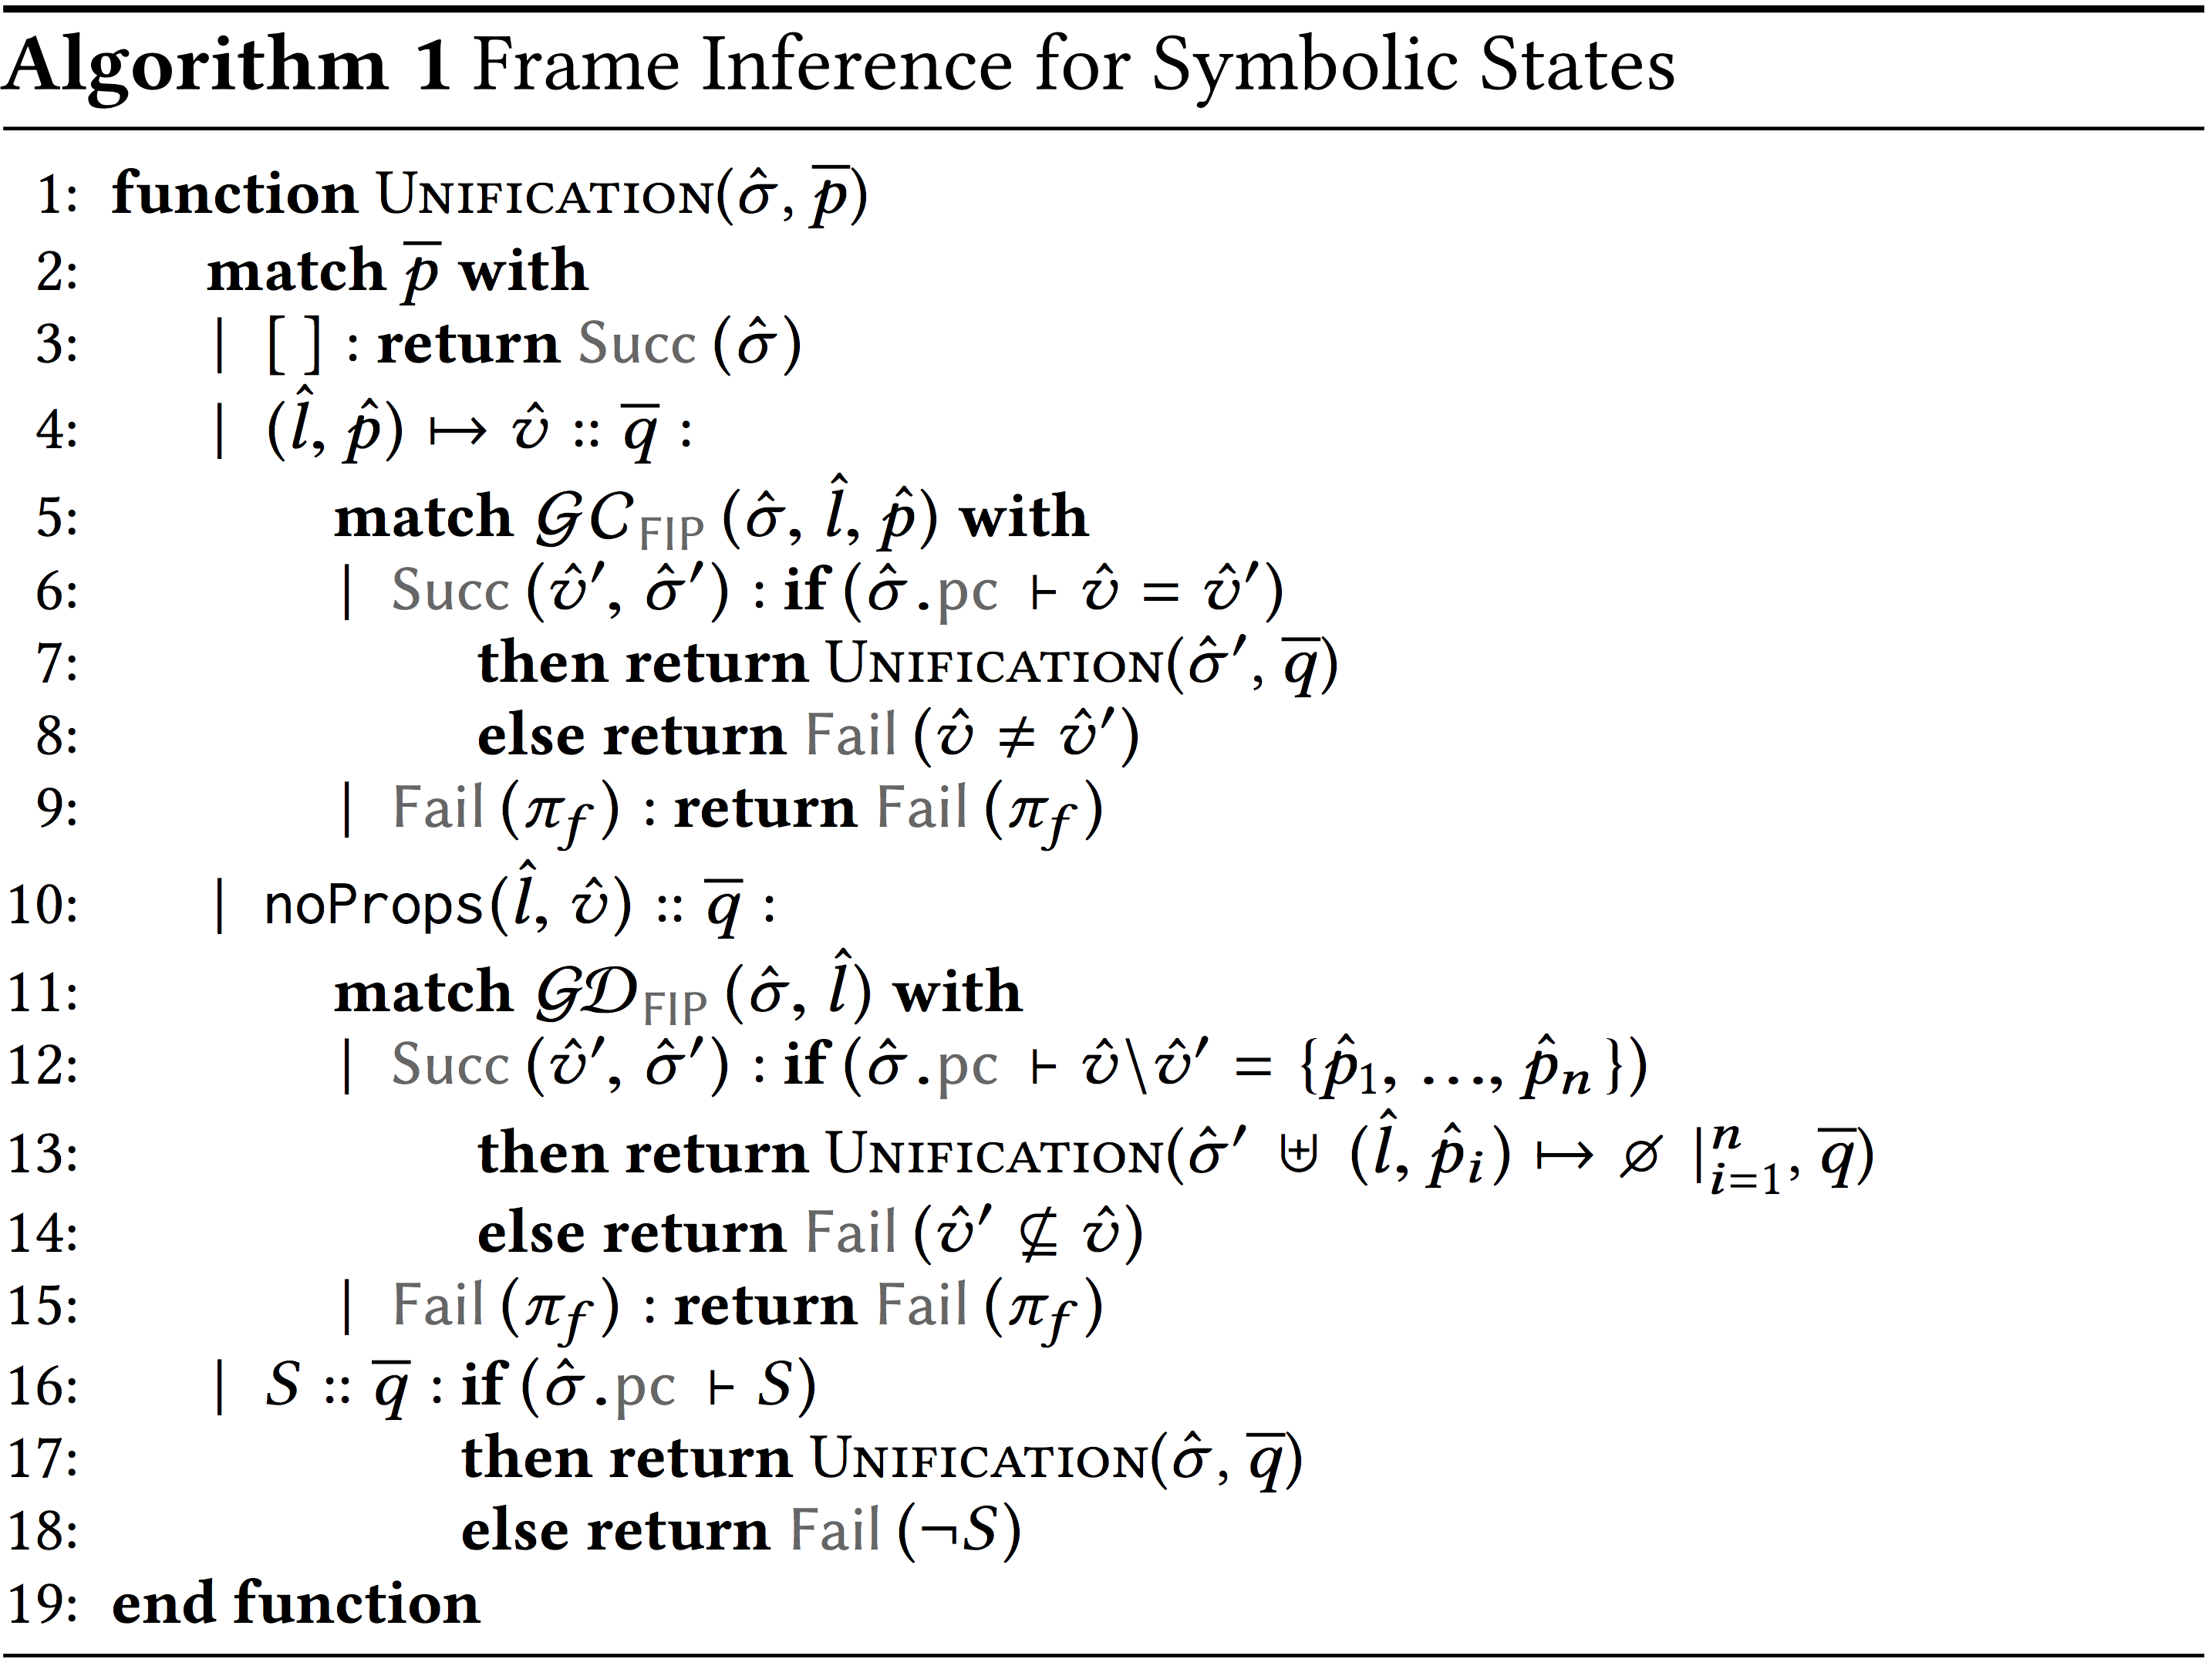
\includegraphics[width=0.47\textwidth]{figures/algorithm.png}
\vspace*{-0.5cm}
\end{figure}

%\vspace*{-0.8cm}

\myparagraph{Example: Unification Algorithm}
Let $\sstate=(\storeemp, \sheap, \sdom, \jtrue)$, where $\sheap = [\hcell{\sloc}{\sexprp_1}{\sexprv}]$ and $\sdom = [ \sloc \mapsto \{ \sexprp_1 \}]$. If the next assertion to be unified is $\emptyfields{\loc}{\{ \sexprp_1 \}}$, the unification will succeed due to the \prooflab{GetDomain} rule. The heap of the resulting symbolic state will be equal to $\sheap$ and the domain table will be empty. On the other hand, if the next assertion is $\emptyfields{\loc}{\{ \sexprp_2 \}}$, the unification will fail. The \prooflab{GetDomain} rule will return $\sexprv' = \{ \sexprp_1 \}$, but since we have no information on $\sexprp_2$, we will not be able to determine the set difference $\sexprv'\backslash\sexprv$ and will fail with the failing constraint $\{ \sexprp_2 \} \subsetneq \{ \sexprp_1 \}$.

\myparagraph{Formal Guarantees} 
%Both our simplified $\unificationfun(\sstate, \pass)$ PDP, presented here, and its full version, given in the Appendix, satisfy the criteria outlined in \S\ref{subsec:sep:assertions}. 
$\unificationfun(\sstate, \pass)$ meets the criteria 
outlined in~\S\ref{subsec:sep:assertions}.

\begin{theorem}[Soundness of FIP]\label{teo:fip:soundness} 
The following hold: 
\begin{enumerate}%[leftmargin=*]
\setlength{\itemsep}{0.1cm}
\item $\unificationfun(\sstate, \pass) = \success{\sstate_f}
        \implies 
        \interpret{}{}(\sstate) \subseteq \interpret{}{}(\sstate_f \statecompose \normaliser(\pass))$
 \item  $\unificationfun(\sstate, \pass) = \fail{\pc_f} 
   \implies
   \interpret{}{}(\sstate \, \wedge \, \pc_f) \cap \interpret{}{}(\pass) = \emptyset$
\end{enumerate}
\end{theorem}

%\begin{theorem}[Bug-finding for SL]\label{teo:fip:bugfinding}

\subsection{From Specifications to Symbolic Tests}\label{specs:to:symbolic:tests}

\jsil Logic specifications have the form $\specsig{\pass}{\pid(\jvec{x})}{\qass}{\flag}$, where $\pass$ and $\qass$ are the 
pre- and postconditions of the procedure with identifier $\pid$ and formal parameters $\jvec{x}$. 
Each specification is associated with a return mode $\flag \in \{ \fnormal, \ferror \}$, indicating if the function
 returns normally or with an error. 
 %If it returns normally, then its return value can be accessed  via a dedicated variable 
% $\retvar$, and $\errvar$ otherwise. 
 Intuitively, a specification $\specsig{\pass}{\pid(\jvec{x})}{\qass}{\flag}$ is 
valid for a given \jsil program $\prog$, if $\prog$ contains a procedure with identifier 
$\pid$ and ``whenever $\pid$ is executed in a state satisfying $P$, then, 
if it terminates, it does so in a state satisfying $Q$, with return mode~$\flag$''.
The formal definition is given below. 


\begin{definition}[Validity of \jsil Logic Specifications]
A \jsil logic specification $\specsig{\pass}{\pid(\jvec{x})}{\qass}{\flag}$ is valid with respect to a program 
$\prog$, written $\prog \satisfies \specsig{\pass}{\pid(\jvec{x})}{\qass}{\flag}$, if and only if it holds that: 
$$
\begin{array}{l}
   (\jstate, \heap_f) \in \interpret{}{}(P) 
   \ \wedge \ 
    \transabssemrule{\jstate \dunion \heap_f, \cs, 0}{\jstate', \cs, i_{\flag'}}{\top}{\top}{\concrete} \\ \quad \
   \implies
      \flag' = \flag \ \wedge \ \exists \jstate'' \, . \, \jstate' = \jstate'' \dunion \heap_f
          \ \wedge \   (\jstate'', \heap_f) \in \interpret{}{}(Q) 
\end{array}
$$
for any call stack $\cs$ of the form $(\pid, -, -, -, -) :: -$. 
\end{definition}

%\pmax{Should that concrete transition have a star?}

\begin{figure}
{\footnotesize
$$
\begin{array}{lll}
\testify{}(\specsig{P}{\pid(\jvar_0, ..., \jvar_n)}{Q}{\flag}) \ \semeq                           &  \testify{\fnormal}(\pid, \svar_i|_{i=0}^n, Q) \ \semeq \\
%
\quad  \mathbf{let} \ \sstore =  [ \jvar_i \mapsto \svar_i|_{i=0}^n] \ \mathbf{in}        &  \quad \darkmath{\sf proc} \jsilmain () \{    \\
%
\quad  \mathbf{let} \ \sstate = \normaliser(\sstore(P)) \ \mathbf{in}                               &   \qquad 0_{\phantom{\sf nm}}: \jsilcall{\jvar}{\pid}{\svar_0, ..., \svar_n}{\errlab} \\
 %
\quad  \mathbf{let} \ Q' = \sstore(Q) \ \mathbf{in}                                                           &  \qquad \retlab \, : \sepassert(Q[\jvar/\retvar])  \\
 %
\quad  \mathbf{let} \ \proc = \testify{\flag}(\pid, \svar_i|_{i=0}^n, Q')  \ \mathbf{in}  &    \qquad \errlab \, \, \, : \jassert(\jfalse)   \\
 %
\qquad (\proc, \sstate)                                                                                                 &  \quad \}  
\end{array}
$$}
\vspace*{-0.4cm}
\caption{\small Symbolic Test Generation Algorithm~\label{fig:test:generation}}
\vspace*{-0.6cm}
\end{figure}

Given a \jsil program $\prog$ containing a procedure $\pid$ with specification {\small $\specsig{\pass}{\pid(\jvec{x})}{\qass}{\flag}$}, 
our goal is to construct a symbolic test for checking if $\pid$ behaves as its specification mandates.
A symbolic test is a pair $(\proc, \sheap)$ consisting of a \jsil procedure with the code of the test and the initial 
symbolic heap on which to execute the test. 
%
Figure~\ref{fig:test:generation} presents the test generation procedure. 
%Intuitively, $\testify{}(\specsig{\pass}{\pid(\jvec{x})}{\qass}{\flag})$ 
%returns the symbolic test for $\specsig{\pass}{\pid(\jvec{x})}{\qass}{\flag}$. 
The test generation function $\testifyfun{} \ $ is defined in terms 
of two auxiliary functions, $\testifyfun{\fnormal}$ and $\testifyfun{\ferror}$, for generating tests for $\fnormal$-mode and 
$\ferror$-mode specifications, respectively. 
For space reasons, we only present $\testifyfun{\fnormal}$ ($\testifyfun{\ferror}$ is equivalent). 
The test program $\prog'$, denoted by $\prog[\jsilmain \mapsto \proc]$, is obtained from the original program $\prog$ and the test procedure $\proc$ by replacing the 
$\jsilmain$ of $\prog$ with the new test procedure, $\proc$. 

\myparagraph{Formal Guarantees}
If the symbolic execution of a 
test generated for $\specsig{\pass}{\pid(\jvec{x})}{\qass}{\flag}$ finds a bug, the specification 
is not~valid.

\begin{theorem}[Bug-finding for \jsil SL Specifications]\label{teo:bug:finding:sl}
$$
\begin{array}{l}
\testify{}(\specsig{\pass}{\pid(\jvec{x})}{\qass}{\flag})  = (\proc, \sstate) \, \wedge \\
\quad
  \prog[\jsilmain \mapsto \proc] :  \transabssemrule{\sstate, \csmain, 0}{-, -, -}{\top}{\bot}{\symbolic} \\ \quad \qquad 
    \implies  
         \prog \not\satisfies \specsig{\pass}{\pid(\jvec{x})}{\qass}{\flag}
\end{array}
$$
%\noindent where  $\csmain = [ \jsilmain, -, -, -, - ]$.
\end{theorem}


\subsection{Lifting the results to JavaScript}\label{subsec:liftmejs2}

\javert specifications of JS functions are analogous to \jsil specifications of \jsil procedures.
%, and are of the form $\specsig{P_{\jssubscript}}{\pid(\jvec{x})}{Q_{\jssubscript}}{\flag}$. 
A \javert specification $\specsig{P_{\jssubscript}}{\pid(\jvec{x})}{Q_{\jssubscript}}{\flag}$
is valid for a JS program $\jstmt$, written $\jstmt \satisfies \specsig{P_{\jssubscript}}{\pid(\jvec{x})}{Q_{\jssubscript}}{\flag}$ if and only if $\jstmt$ contains a function literal with identifier $\pid$ and ``whenever $\pid$ is executed in a state satisfying $P_\jssubscript$, then, 
if it terminates, it does so in a state satisfying $Q_\jssubscript$, with return mode $\flag$''. 
%The assertion language used by \javert is very similar to the assertion language of \jsil and is described in detail in~\cite{javert}.
\JSComp is proven to correctly compile \javert specifications to \jsil specifications~\cite{javert}.

\myparagraph{Testing \javert Specifications}
We generate symbolic tests from a JS program and its \javert specifications by: converting them to a \jsil program with \jsil specifications, using \jstojsil; generating a set of symbolic tests from the obtained \jsil program and \jsil specifications, as described in \S\ref{specs:to:symbolic:tests}; and running the generated \jsil symbolic tests using the \jsil symbolic semantics described in \S\ref{subsec:symb:semantics}. 
If \cosette finds a bug while running the tests, we will obtain a concrete counter-example triggering a specification violation.

\myparagraph{Formal Guarantees}
The correctness of \JSComp ensures that 
%the analysis of \jsil programs can be lifted to JavaScript programs. More concretely,
%
 a \javert  specification $\specsig{P_{\jssubscript}}{\pid(\jvec{x})}{Q_{\jssubscript}}{\flag}$
is valid for a given JS program $\jstmt$ \emph{iff} the translated specification 
$\compile(\specsig{P_{\jssubscript}}{\pid(\jvec{x})}{Q_{\jssubscript}}{\flag})$ is valid 
for the compilation of $\jstmt$.
Hence, we can lift Theorem~\ref{teo:bug:finding:sl} to the JavaScript level in a straightforward way, 
as shown below. 

\begin{corollary}[Bug-finding for \javert Specifications]\label{teo:bug:finding:sl:javert}
$$
\begin{array}{l}
\testify{}(\compile(\specsig{\pass_\jssubscript}{\pid(\jvec{x})}{\qass_\jssubscript}{\flag}))  = (\proc, \sstate) \, \wedge \\
\quad
  \compile(\jstmt)[\jsilmain \mapsto \proc] :  \transabssemrule{\sstate, \csmain, 0}{-, -, -}{\top}{\bot}{\symbolic} \\ \quad \qquad 
    \implies  
         \jstmt \not\satisfies \specsig{\pass_\jssubscript}{\pid(\jvec{x})}{\qass_\jssubscript}{\flag}.
\end{array}
$$
\end{corollary}


%
%
%\javert specifications of JS functions are analogous to \jsil specifications of \jsil procedures.
%%, and are of the form $\specsig{P_{\jssubscript}}{\pid(\jvec{x})}{Q_{\jssubscript}}{\flag}$. 
%As for \jsil, a \javert~\cite{javert} specification $\specsig{P_{\jssubscript}}{\pid(\jvec{x})}{Q_{\jssubscript}}{\flag}$
%is valid for a JavaScript program $\jstmt$, written $\jstmt \satisfies \specsig{P_{\jssubscript}}{\pid(\jvec{x})}{Q_{\jssubscript}}{\flag}$, 
%if and only if $\jstmt$ contains a function literal with identifier $\pid$ and ``whenever $\pid$ is executed in a state satisfying $P_\jssubscript$, then, 
%if it terminates, it does so in a state satisfying $Q_\jssubscript$, with return mode $\flag$''. 
%%The assertion language used by \javert is very similar to the assertion language of \jsil and is described in detail in~\cite{javert}.
%\javert comes with a proven correct compiler from \javert specifications to \jsil specifications, denoted by $\jsspeccomp$. 
%
%\myparagraph{Testing \javert Specifications}
%We generate symbolic tests from JavaScript programs and their \javert specifications in the following way. 
%First, we convert the JavaScript program and its \javert specifications to a \jsil program with \jsil specifications, 
%using \jstojsil and $\jsspeccomp$. Next, we generate a set of symbolic tests from the obtained 
%\jsil program and \jsil specifications, as described in \S\ref{specs:to:symbolic:tests}. 
%Finally, we run the generated \jsil symbolic tests using the \jsil symbolic semantics described on \S\ref{subsec:symb:semantics}. 
%If \cosette finds a bug while running these tests, we will obtain a concrete counter-example triggering that bug.
%
%\myparagraph{Formal Guarantees}
%The correctness proof ensures that the verification of \jsil programs can be lifted to the verification of JavaScript programs.
%%
%More concretely, a \javert  specification $\specsig{P_{\jssubscript}}{\pid(\jvec{x})}{Q_{\jssubscript}}{\flag}$
%is valid for a given JavaScript program $\jstmt$ if and only if the translated specification 
%$\jsspeccomp(\specsig{P_{\jssubscript}}{\pid(\jvec{x})}{Q_{\jssubscript}}{\flag})$ is valid 
%for the compilation of $\jstmt$ by a correct compiler $\compile$. 
%



